\documentclass{article}
\usepackage{arxiv}

\usepackage[utf8]{inputenc}
\usepackage[english, russian]{babel}
\usepackage[T1]{fontenc}
\usepackage{url}
\usepackage{booktabs}
\usepackage{amsfonts}
\usepackage{nicefrac}
\usepackage{microtype}
\usepackage{lipsum}
\usepackage{graphicx}
\usepackage{natbib}
\usepackage{doi}



\title{Выделение элементов реакции на электроэнцефалограмме}

\author{ Никишкина Евгения Геннадьевна \\
        \texttt{nikishkina.jane@gmail.com} \\
	Московский государственный университет имени М. В. Ломоносова\\
    Научный руководитель: Майсурадзе Арчил Ивериевич \\
	%% examples of more authors
	} \\
	%% \AND
	%% Coauthor \\
	%% Affiliation \\
	%% Address \\
	%% \texttt{email} \\
	%% \And
	%% Coauthor \\
	%% Affiliation \\
	%% Address \\
	%% \texttt{email} \\
	%% \And
	%% Coauthor \\
	%% Affiliation \\
	%% Address \\
	%% \texttt{email} \\
}
\date{}

\renewcommand{\shorttitle}{\textit{arXiv} Template}

%%% Add PDF metadata to help others organize their library
%%% Once the PDF is generated, you can check the metadata with
%%% $ pdfinfo template.pdf
\hypersetup{
pdftitle={Выделение элементов реакции на электроэнцефалограмме},
pdfsubject={Machine Learning},
pdfauthor={Никишкина Евгения Геннадьевна},
pdfkeywords={First keyword, Second keyword, More},
}

\begin{document}
\maketitle

\begin{abstract}
	Изменения в эмоциональном состоянии человека могут влиять на сигналы электроэнцефалограммы (ЭЭГ). Распознавание и анализ эмоций с использованием биологических сигналов мозга является сложной задачей, требующей точной обработки и выделения признаков для определения наличия эмоции у конкретного человека. Целью данной работы было создание эффективного алгоритма для распознавания эмоций человека на основе анализа рядов ЭЭГ. Были проанализированы различные подходы, в результате чего был выбран оптимальный метод, который затем был реализован в собственной программе. Также были проведены эксперименты на основе подобранных рядов ЭЭГ, содержащих данные об эмоциональных состояниях. Для детектирования эмоций в рядах ЭЭГ был использован новый подход, основанный на анализе аномалий. Результаты экспериментов продемонстрировали, что разработанный алгоритм позволяет получать интерпретируемые результаты по определению наличия эмоций у человека.
\end{abstract}


\keywords{Электроэнцефалография (ЭЭГ) \and Временный ряды \and Детектирование аномалий \and Распознавание эмоций \and SEED dataset \and Глубинное обучение} 

\section{Введение}
Эмоции представляют собой проявления не только физиологических состояний, связанных с разнообразными чувствами, мыслями и поведением людей, но и психологических откликов на множество внешних стимулов. Умение точно распознавать эмоции играет ключевую роль во множестве сфер: взаимодействие человека и компьютера (HCI) \citep{HCI}, здравоохранение \citep{healtcare}, интернет-образование \citep{inted}, мониторинг безопасности \citep{security}, психологический анализ \citep{psych}, а также индустрия развлечений \citep{entern}. Например, распознавание эмоций может оказаться весьма полезным для диагностики таких психических заболеваний, как депрессия и шизофрения \citep{schizophrenia}. Также при взаимодействии человека с компьютером извлеченные эмоции могут использоваться как своего рода обратная связь для предоставления лучшего контента, улучшающего пользовательский опыт в электронном обучении, компьютерных играх и поиске информации (\citep{HCI}).

В последние годы существующие модели распознавания эмоций были разделены на две категории: методы, основанные на физиологических сигналах, и методы, основанные на нефизиологических сигналах \citep{sensors18}. По сравнению с нефизиологическими сигналами, физиологические сигналы не восприимчивы к субъективным факторам, которые могут достоверно отображать эмоциональные состояния человека. Таким образом, распознавание эмоций, основанное на физиологических сигналах, имеет большие преимущества в надежности и практичности\citep{sensors}. Временной ряд представляет собой собранный в разные моменты времени статистический материал о значении каких-либо параметров исследуемого процесса \citep{time_series}. Каждая единица статистического материала называется измерением или отсчётом, причем для каждого отсчёта должно быть указано время или порядковый номер измерения. Важно отметить, что при анализе временного ряда учитывается взаимосвязь измерений со временем, что отличает его от простой выборки данных, где учитывается только статистическое разнообразие и характеристики выборки. В области исследований, основанных на физиологических сигналах, ЭЭГ - это спонтанный, несубъективный физиологический сигнал, который может объективно отражать эмоциональные состояния человека \citep{eeg}. В данной работе объектом исследования являются реальные временные ряды, а именно, — записи электроэнцефалограммы. Электроэнцефалография (ЭЭГ) является методом исследования электрической активности мозга путем размещения электродов в определенных зонах на поверхности головы. Данные, полученные таким образом, представляют собой многомерный временной ряд (каждый датчик отвечает за одномерный временной ряд), то есть система из нескольких одномерных рядов, где целевые значения зависят не только от предыдущих значений одного временного ряда, но и от значений дополнительных временных рядов \citep{seed}.

Методы распознавания эмоций на основе ЭЭГ можно разделить на две группы: методы классического машинного обучения и глубокого обучения \citep{sensors18}. В методах распознавания эмоций, основанных на классическом машинном обучении, признаки извлекаются вручную для последующего использования в статистических методах, метрических, модельных методов, таких как, например, метод опорных векторов (SVM) \citet{scholkopfsuppor} и Isolation Forest \citet{liu2008isolation}. Лин и др. \citet{sensors18} представили общий процесс традиционных методов машинного обучения для распознавания эмоций по ЭЭГ, включая регистрацию эмоций, получение сигнала, выделение признаков, последующие распознавание или классификация эмоций и т.д. Однако, с такими подходами возникает проблема: из-за нелинейности и высокой размерности сигналов ЭЭГ, методы, эффективные на линейных и низкоразмерных данных, не обеспечивают высокое качество решения сложных задач. Также данные подходы имеет существенный недостаток, заключающийся в том, что процесс извлечения признаков обычно затруднителен и в значительной степени зависит от экспертов-людей. Трудно получить все подразумеваемые признаки путем извлечения вручную, и используемые формулы часто очень сложны. Кроме того, сигналы ЭЭГ чувствительны к шумам, таким как электромиографические артефакты, которые создают серьезные помехи. Ввиду вышеуказанных трудностей для решения этих проблем используются некоторые методы глубокого обучения. Альхагри и др. \citep{lstm} предложили LSTM для изучения особенностей по сигналам ЭЭГ, затем в качестве классификатора используется полносвязный слой. Для оценки представленного метода использовался набор данных DEAP, на котором предложенный метод дает среднюю точность $85,65\%$, $85,45\%$ и $87,99\%$ для классов возбуждения, валентности и симпатии соответственно. Предложенный метод обеспечил высокую среднюю точность по сравнению с традиционными методами. Ширрмейстер и др. \citep{cnn} использовали сверточные нейронные сети (CNN) для декодирования и визуализации ЭЭГ, которые продемонстрировали большой потенциал при применении к сквозному распознаванию эмоций на основе ЭЭГ-сигналов, тем самым подтвердив превосходство глубоких нейронных сетей в задачах классификации ЭЭГ. В последние годы CNN (\citep{sensors_cnn}, \citep{med_cnn}), LSTM (\citep{lstm}, \citep{sharma}), Generative Adversarial Network (GAN) (\citep{gan}) и другие сетевые модели широко использовались при распознавании эмоций по ЭЭГ.

\section{Постановка задачи}
Дан многомерный временной ряд длины $n$ $X = \{x_1, x_2, x_3, ..., x_n\}$, где каждый элемент $x_t \in \mathbb{R}^{m}$ - $m$-мерный вектор, представляющий собой показания $m$ датчиков в момент времени $t$. Пусть  дана обучающая выборка, которая представляет собой многомерные временные ряды для $\widetilde{n}$, полученные по участникам эксперимента, находящимся в безэмоциональном состоянии. Необходимо для исходного временного ряда предсказать $Y = \{y_1, y_2, y_3, ..., y_n\}$, где каждый элемент $y_t \in \{0, 1\}^{m}$ -- $m$-мерный вектор, определяющий для каждого из $m$ датчиков аномальность показания в момент времени $t$. Будем считать, что момент времени $t$ аномальный, если показание хотя бы одного из $m$ датчиков является аномальным. Таким образом, получим вектор $\widetilde{Y} = \{\widetilde{y_1}, \widetilde{y_2}, \widetilde{y_3}, ..., \widetilde{y_n}\}$, где элемент $\widetilde{y_t} \in \{0, 1\}$ (1 отвечает за аномальность). \\
Для тестовых данных для каждой временной точки на основе порога (алгоритм POT) можно получить ответ алгоритма --- является ли данная точка аномальной или нет. Разметка для сигналов ЭЭГ отсутствует, поэтому для оценки качества используется косвенная метрика: на основе меток аномальности, полученных алгоритмом, для положительных и нейтральных видео в тестовых данных можно посчитать процент аномальных точек в нем; данную величину можно рассматривать в качестве оценки принадлежности объекта (то есть временного ряда ЭЭГ для конкретного видео) к классу нейтральных данных; на основе этих оценок можно воспользоваться метриками для задачи бинарной классификации (в данной работе была выбрана метрика AUC-ROC).

\section{Эксперименты}
\subsection{Данные}
Эксперименты проводились на датасете SEED \cite{seed}. При создании данного датасета были выбраны пятнадцать фрагментов китайских фильмов, характеризующие положительные, нейтральные и отрицательные эмоции в качестве стимулов, использованных в экспериментах. Критерии отбора видеоклипов следующие:
\begin{itemize}
    \item продолжительность всего эксперимента не должна быть слишком большой, чтобы не вызвать у испытуемого усталость;
    \item  видеоролики должны быть понятны без объяснений;
    \item видеоролики должны вызывать единственную желаемую целевую эмоцию.
\end{itemize}
Продолжительность каждого фрагмента фильма составляет примерно 4 минуты. Каждый видеоклип отредактирован так, чтобы создать связную эмоцию, вызывающую интерес, и максимизировать эмоциональный смысл. 

В экспериментах принимали участие пятнадцать китайских испытуемых (7 мужчин и 8 женщин). Для каждого эксперимента предусмотрено в общей сложности 15 испытаний. Перед каждым клипом была 5-секундная подсказка о начале, 45 секунд для самостоятельной оценки и 15 секунд для отдыха после каждого клипа в течение одного сеанса. Порядок представления организован таким образом, что два фрагмента фильма, отвечающих за одну и ту же эмоцию, не показываются последовательно. Для получения обратной связи участникам было предложено сообщить о своих эмоциональных реакциях на каждый фрагмент фильма, заполнив анкету сразу после просмотра каждого ролика. Сигналы ЭЭГ регистрировались с помощью 62-канальной системы ESI NeuroScan. Сцена эксперимента и соответствующее расположение электродов для ЭЭГ показаны ниже.

\begin{figure}[h]
\begin{tabular}{cc}
  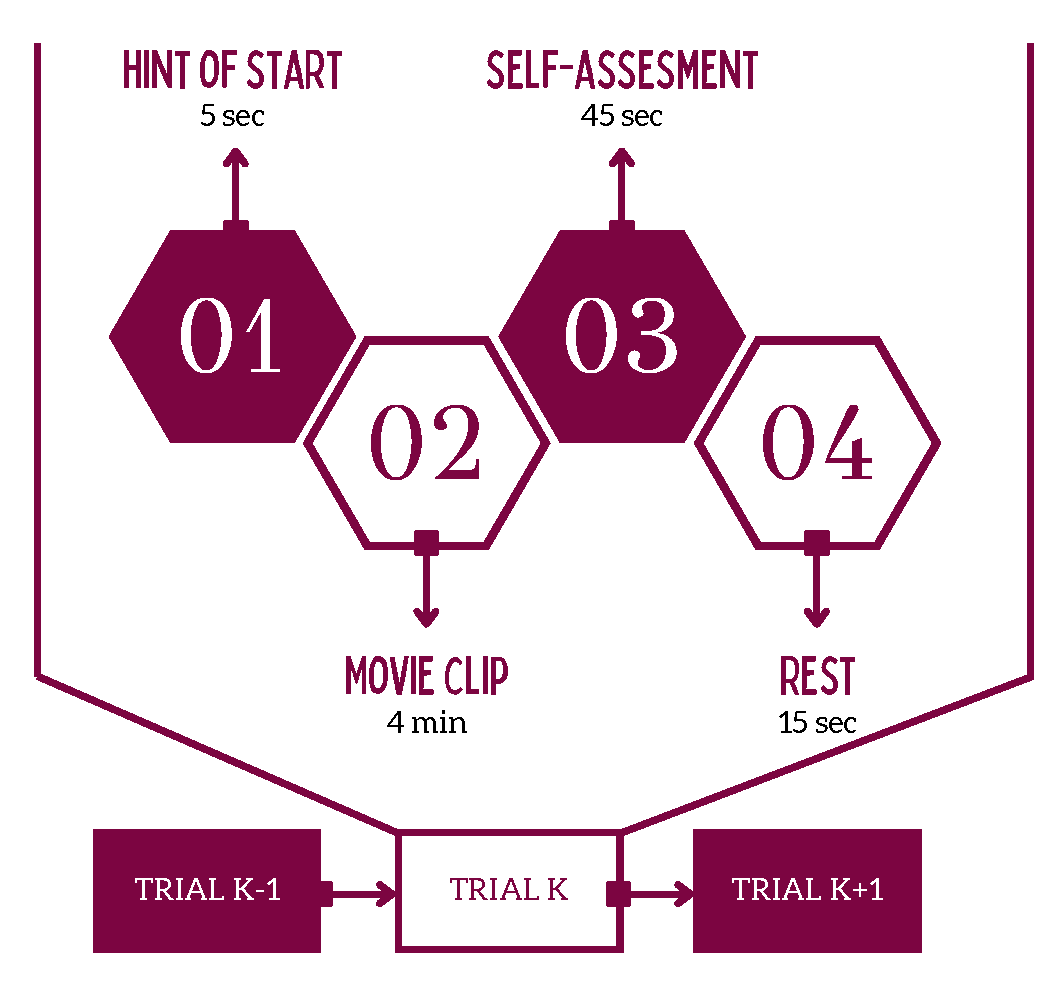
\includegraphics[width=75mm]{1.pdf} &   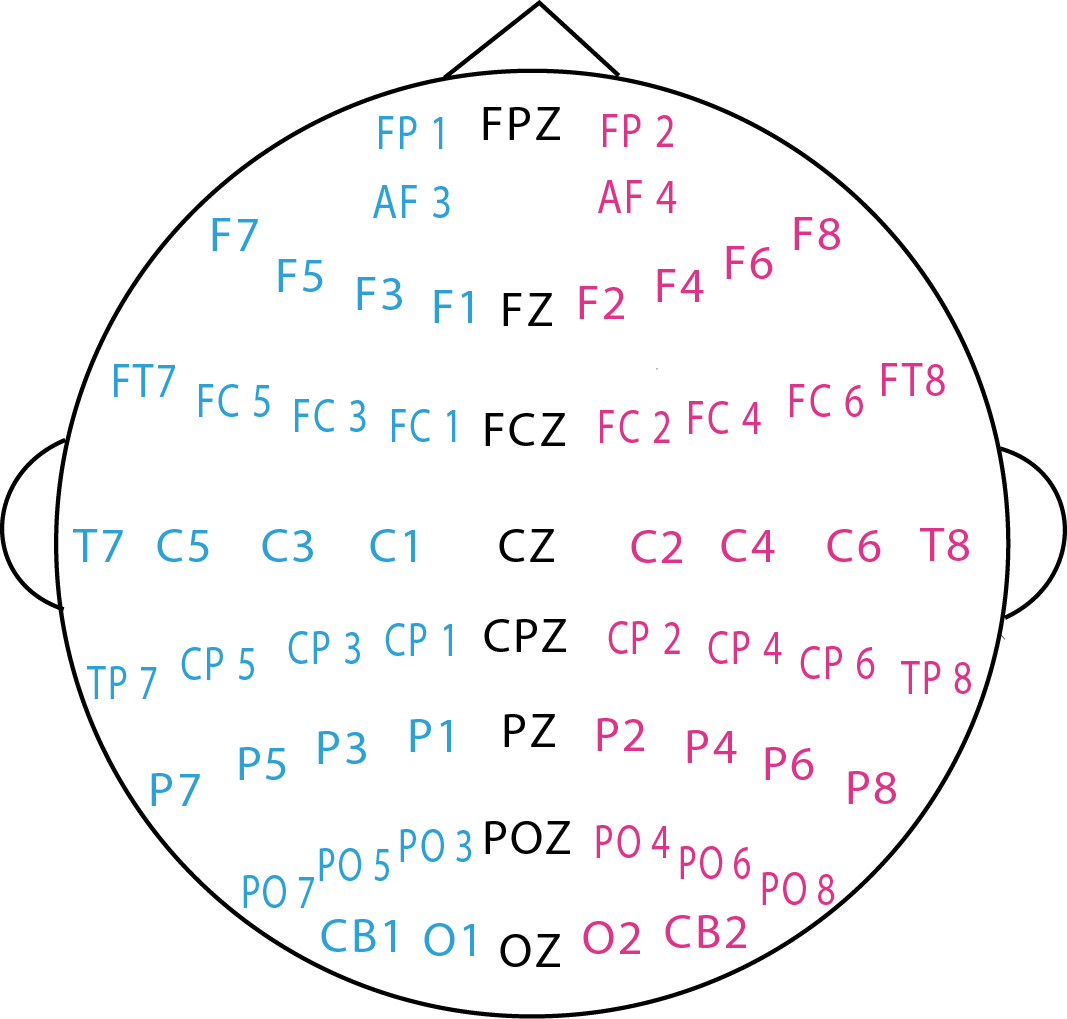
\includegraphics[width=75mm]{2.png} \\
\end{tabular}
\caption{Сцена эксперимента и расположение электродов для ЭЭГ}
\end{figure}

Данные представляют собой файлы, содержащие уменьшенные, предварительно обработанные и сегментированные показания ЭЭГ в MATLAB (файл .mat). Частота была уменьшена до 200 Гц., также был применен полосовой фильтр (BPF) с частотой от 0 до 75 Гц, после чего были извлечены сегменты ЭЭГ, соответствующие продолжительности каждого фрагмента фильма. 
Каждый испытуемый принимал участие в эксперименте три раза с интервалом примерно в одну неделю. Для одного эксперимента было предусмотрено 15 испытаний (1 испытание — просмотр одного видеоролика). Таким образом, для каждого участника эксперимента было получено 45 файлов с расширением .mat, по одному на каждое испытание. 

\subsection{Вычислительные эксперименты}

Для того чтобы смоделировать локальную зависимость данных в точке $x_t$ в момент времени $t$ необходимо взять окно длины $K$: 
$$
W_t = \{x_{t - K + 1}, \dots, x_t\}.
$$
Таким образом, весь временной ряд $\textit{T}$ преобразуется в последовательность скользящих окон $\textit{W} = \{W_1, \dots, W_T\}$. Для случая $t < K$ первый элемент временного ряда дублируется такое число раз, чтобы длина окна стала равна $K$. Помимо этого с целью восстановления долгосрочных взаимосвязей необходимо также рассматривать временной отрезок до текущей временной метки $t$ ряда $\textit{T}$ (обозначим его $C$).
\subsection{Базовый эксперимент}
\begin{figure}[h]
\begin{tabular}{cc}
  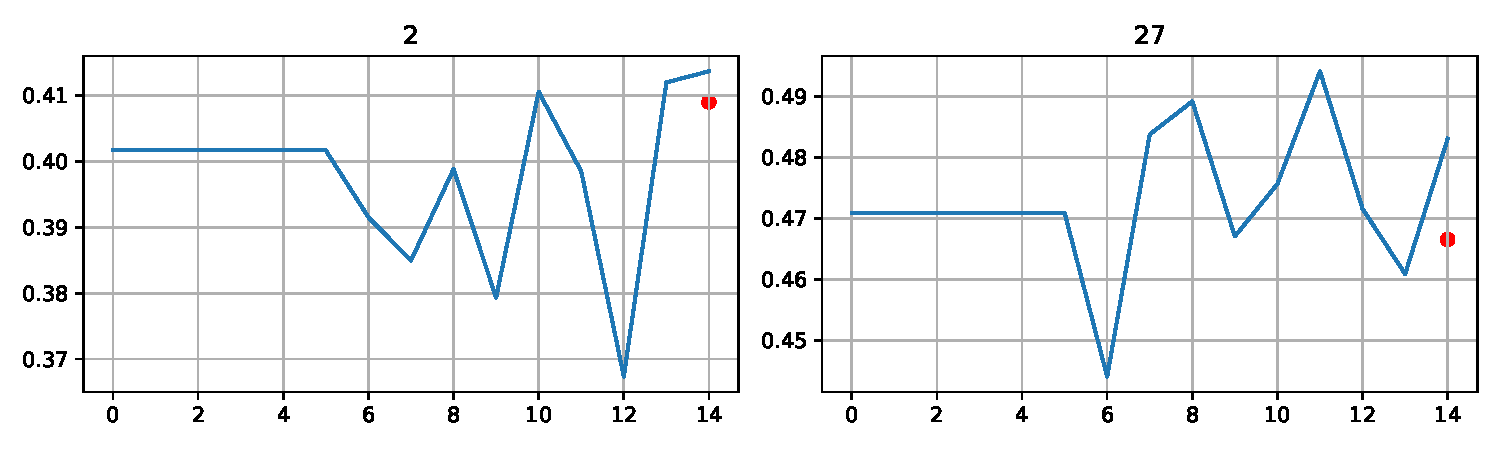
\includegraphics[width=160mm]{5.pdf} 
\end{tabular}
\caption{Полученные результаты предсказания для 2-ого и 27-ого датчиков}
\label{fig:base}
\end{figure}

\begin{figure}[h]
\begin{tabular}{cc}
  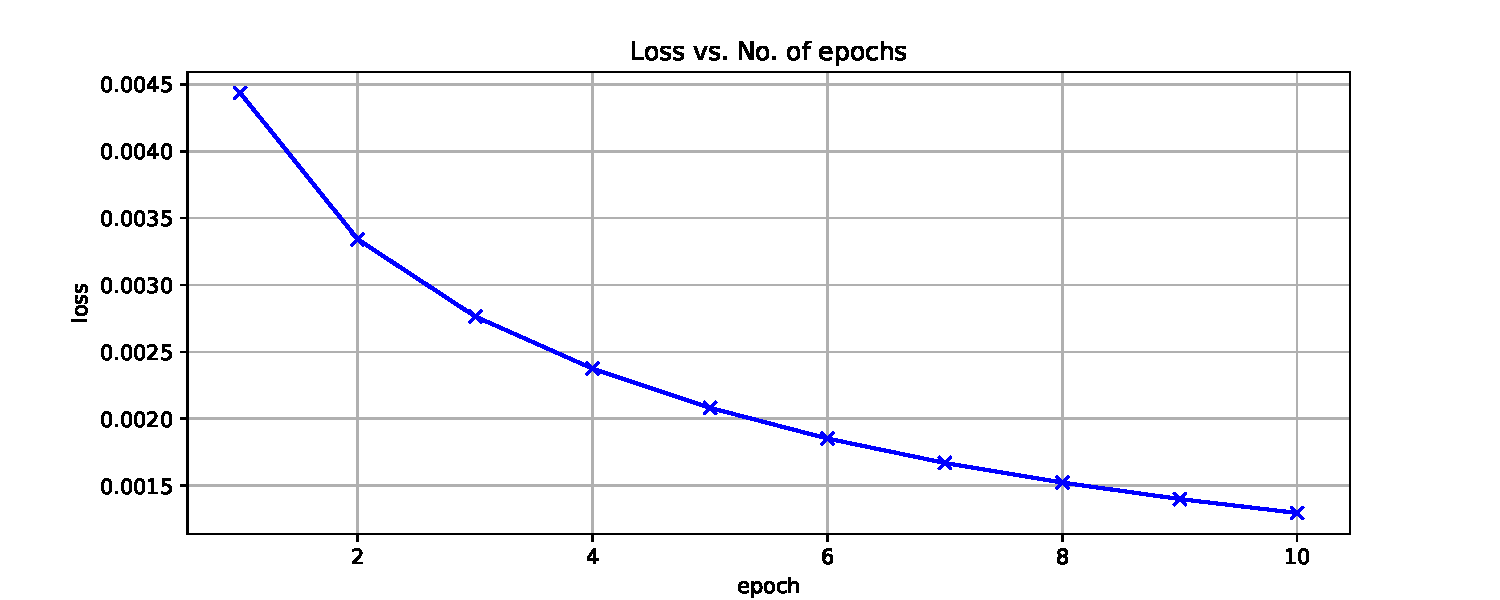
\includegraphics[width=160mm]{6.pdf} 
\end{tabular}
\caption{Зависимость ошибки от номера эпохи на обучении}
\label{fig:base_mse}
\end{figure}

В качестве базовой модели была взята простая нейросетевая архитектура, состояшая из двух полносвязных слоев и функции активации ReLU. 

Обучение состоит в предсказании следующий точки временного ряда, на основе фиксированного количества $K - 1$ предыдущих точек данного временного ряда. Модель обучается на данных, отвечающих нейтральным эмоциям на задачу минимизации среднеквадратичной ошибки MSE. На рисунке \ref{fig:base} представлено предсказание $K$-ой метки временного ряда на основе предыдущих для 2-ого и 27-ого датчика.

На основе такого подхода при получении результатов для вновь поступившего временного ряда, отвечающего яркой эмоции, то есть положительной или отрицательной, выдвигается гипотеза, что поскольку обучение происходило на данных, отвечающих нейтральным эмоциям, возможен подбор порога на основе которого мы будем определять наличие эмоции у человека. Модель демонстрирует не самые высокие показатели качества \ref{fig:base_mse}, поэтому стоит обратить внимание на альтернативную модель, способную обеспечивать более высокое качество работы.




\subsection{Основной эксперимент}

Для детектирования аномалий будем использовать модель TranAD \cite{TranAD}. Принцип работы модели схож с принципом работы автокодировщика для детектирования аномалий. Первоначально модель будет переводить переданное на вход окно в пространство меньшей размерности с помощью кодировщика, а затем с помощью декодирощика восстанавливать это окно. Преимущество данного подхода заключается в использовании временного отрезка $С$, который за счет учета долгосрочных тенденций позволяет более точно восстанавливать окно. Также к преимуществам данной модели можно отнести специальную соревновательную процедуру обучения, благодаря которой зашумленные фрагменты предсказываются лучше и не идентифицируются как аномальные.

\subsubsection{Модель трансформер}
В качестве основных блоков в модели используются кодировщих и декодировщик трансформера \cite{attention}. Архитектура модели TranAD представлена на рисунке выше. Для получения представления окна, которое подается на вход декодировщика для его последующего восстановления, используется кодировщик (Window Encoder). 

Пусть размерность временных рядов равна $m$. Необходимо определить стандартные для трансформерных моделей операции. Скалярным вниманием будем называть следующую величину, полученную в результате операций над матрицами $Q$ (запросы), $K$ (ключи) и $V$ (значения): 
$$
\text{Attention}(Q, K, V) = \text{softmax}\big ( \frac{QK^T}{\sqrt{m}} \big )V
$$
В модели TranAD используется многоголовое внимание: 
$$
\text{MultiHeadAtt}(Q, K, V) = Concat(H_1, \dots, H_h)
$$
где $H_i = \text{Attention}(Q_i, K_i, V_i)$. 

Здесь $Q_i$, $K_i$, $V_i$ --- полносвязные слои для каждой из голов трансформера. Дополнительно, чтобы учесть то, что события происходят в разные моменты времени, используется позиционное кодирование \cite{attention}. 

Для обучения модели используется соревновательное обучение наподобие того, что используется в модели GAN. Модель TranAD состоит из двух трансформерных кодировщиков и двух декодировщиков \ref{fig:TranAD}. На вход подаются окно $W$, ряд $C$ и специальная матрица focus score (подробнее про него в секции 4.2.2) $F$, размеры которой совпадают с размерами окна. Матрица F дополняется нулями, производится операция конкатенации полученной матрицы F и ряда $C$, затем применяется позиционное кодирование. Полученная матрица $I_1$ подается на вход первого кодировщика: 
$$
I_1^1 = \text{LayerNorm}(I_1 + \text{MultiHeadAtt}(I_1, I_1, I_1)),
$$
$$
I_1^2 = \text{LayerNorm}(I_1^1 + \text{FeedForward}(I^1_1)). 
$$

\begin{figure}[h]
\begin{tabular}{cc}
  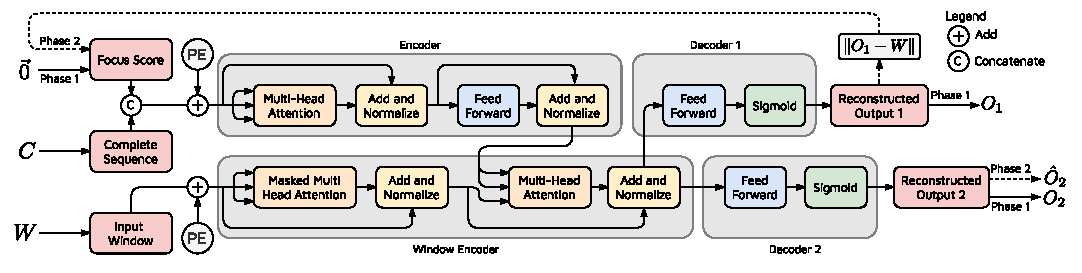
\includegraphics[width=160mm]{3.pdf}
\end{tabular}
\caption{Модель TranAD}
\label{fig:TranAD}
\end{figure}

Перед применением window encoder к окну применяется позиционное кодирование и полученная матрица $I_2$ подается на его вход. При этом здесь используется маскированное <<самовнимание>> (mask self-attention) для того, чтобы декодировщик не мог "подсматривать" \; в будущее во время обучения, то есть во временные точки из будущего в контекстном представлении ряда $C$. Таким образом, window encoder представляет собой: 
$$
I^1_2 = \text{Mask}(\text{MultiHeadAtt}(I_2, I_2, I_2)),
$$
$$
I^2_2 = \text{LayerNorm}(I_2 + I^1_2),
$$
$$
I^3_2 = \text{LayerNorm}(I^2_2 + \text{MultiHeadAtt}(I^2_1, I^2_1, I^2_2)).
$$

То есть контекстные представления всей последовательности $C$ используются в качестве ключей и значений для перекрестного внимания в window encoder. Добавление представления всей последовательности $C$ до момента времени $t$ позволяет модели использовать расширенный контекст. Следующими блоками в модели являются два одинаковых декодировщика, восстанавливающих переданное окно: 
$$
O_i = \text{Sigmoid}(\text{FeedForward}(I^3_2)), i \in \{1, 2\}.
$$
Таким образом, модель TranAD принимает на вход $C$ и $W$ и генерирует два выхода $O_1$ и $O_2$.

\subsubsection{Двухэтапное состязательное обучение}

\begin{figure}[h]
\begin{tabular}{cc}
  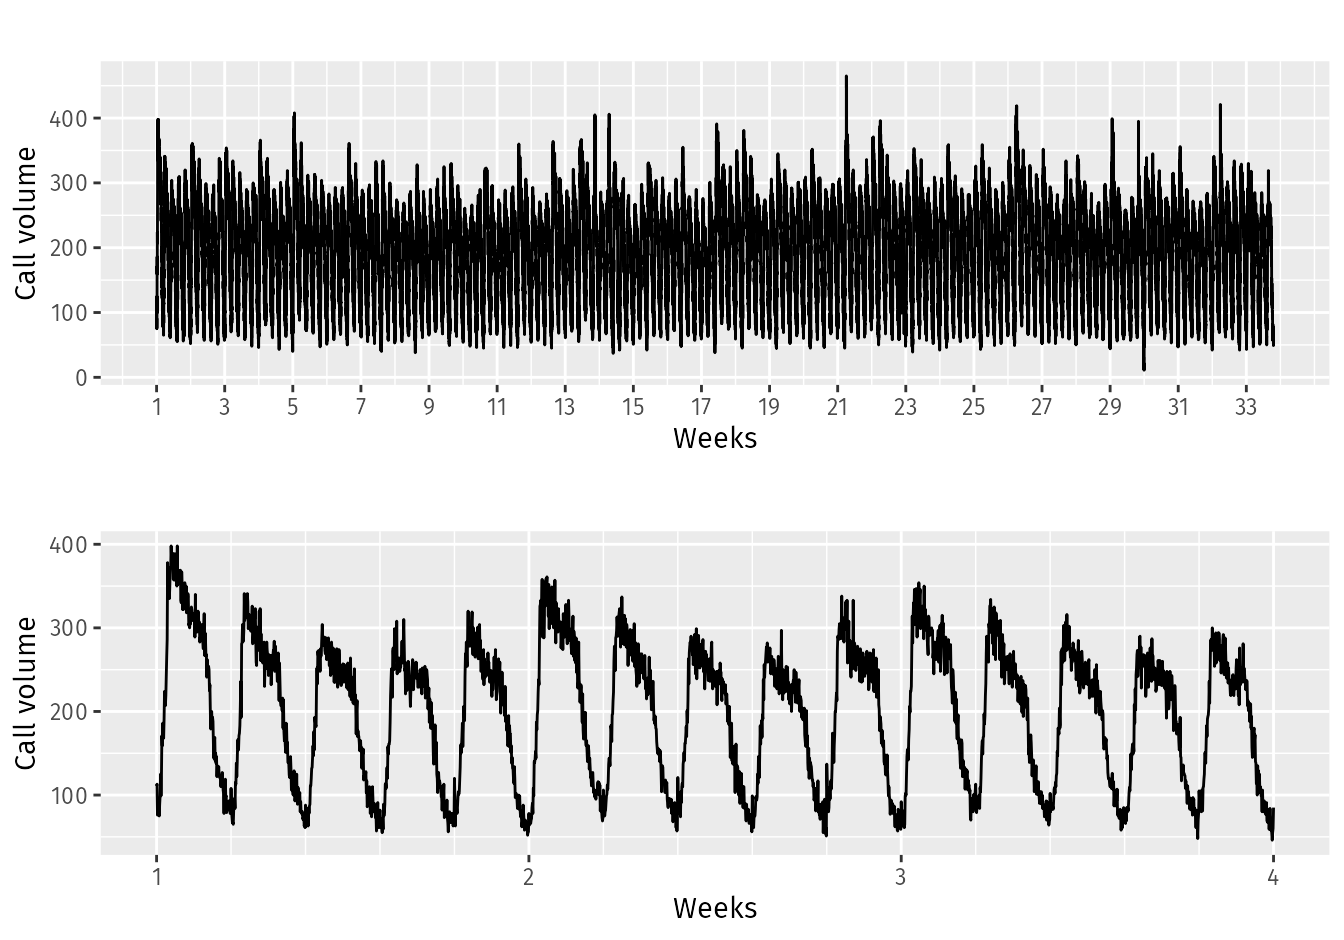
\includegraphics[width=160mm]{4.png}
\end{tabular}
\caption{Пятиминутный объем звонков в крупном североамериканском коммерческом банке}
\label{fig:calls}
\end{figure}

Благодаря учету долгосрочных зависимостей модель способна лучше восстанавливать переданное на вход окно. 

Для того чтобы лучше понять, что имеется в виду, рассмотрим следующий пример. На рисунке \ref{fig:calls} представлены два графика: на первом графике показано количество поступивших звонков в банки с 5-минутным интервалом в промежутке между 7:00 и 21:05 каждого буднего дня в течение 33 недель, на втором показаны первые три недели этого же временного ряда. Знание всей последовательности до текущего момента $t$ дает, например, информацию о времени суток, что в свою очередь, потенциально помогает в восстановлении количества звонков в момент времени $t$. Заметим, что значения количества звонков в дневное время суток более шумные, поэтому модели будет сложнее восстанавливать в данный временной промежуток и она может выдать ложноположительный результат. С целью решения данной проблемы и вводится процедура соревновательного обучения. 


Процедура соревновательного обучения состоит из двух фаз. Первая фаза представляет собой реконструкцию входа модели. Модель пытается сгенерировать входное окно как можно более точно. Поэлементная разность между сгенерированным первым декодером окном и входным окном и есть focus score, о котором было упомянуто выше. Операция конкатенации focus score и входной последовательности облегчает механизму внимания извлекать локальные зависимости, фокусируясь на подпоследовательностях с высокими значениями focus score.  Таким образом, после первой фазы кодировщик преобразует входное окно $W \in \mathbb{R}^{K \times m}$ (с focus score $F = [0]_{K \times m}$) в сжатое представление $I_2^3$, из которого впоследствии получаются выходы $O_1$ и $O_2$. 

Вторая фаза представляет собой реконструкцию входа с использованием focus score. Матрица F, полученная после первой фазы, используется вторым декодером для генерации выхода $\hat{O_2}$. 

Такое двухстадийное авторегрессионное решение имеет ряд преимуществ: 
\begin{enumerate}
    \item Использование focus score уменьшает вероятность появления ложноположительного результата за счет дополнительного настраивания сгенерированного окна на основе ошибок, полученных на первой стадии. 

    \item Соревновательная процедура обучения улучшает обобщающую способность модели, а также помогает модели быть более устойчивой. 
\end{enumerate}

Как было упомянуто ранее, каждый из декодировщиков независимо пытается восстановить входное окно временного ряда. Определим потерю восстановления (reconstruction loss) следующим образом: 
$$
l_1 = ||O_1 - W||_2;
$$
$$
l_2 = ||O_2 - W||_2.
$$
Дополнительно необходимо ввести понятие соревновательной потери (adversarial loss). Во время второй фазы второй декодировщик старается отличить входное окно от окна, сгенерированного первым декодировщиком, путем максимизации $||\hat{O}_2 - W||_2$ (соревновательная потеря). С другой стороны, первый декодировщик старается <<обмануть>> второй декодировщик путем генерации такого окна $O_1$, чтобы focus score был близок к нулю. То есть в процессе обучения нужно оптимизировать следующую величину: 
$$
\min_{Decoder1} \max_{Decoder2} ||\hat{O}_2 - W||_2.
$$

Таким образом, цель первого декодировщика --- минимизировать потерю восстановления, в то время как целью второго является максимизация соревновательной потери. 
$$
l_1 = +||\hat{O}_2 - W||_2;
$$
$$
l_2 = -||\hat{O}_2 - W||_2.
$$
Тогда общая функция потерь будет иметь вид:
$$
L_1 = \frac{1}{n}||O_1 - W||_2 + (1 - \frac{1}{n})||\hat{O}_2 - W||_2;
$$
$$
L_2 = \frac{1}{n}||O_2 - W||_2 - (1 - \frac{1}{n})||\hat{O}_2 - W||_2,
$$
где $n$ --- номер эпохи. На начальных эпохах ошибке восстановления дается большой вес (за вес отвечает множитель $\frac{1}{n}$). Это необходимо для того, чтобы focus score ко второй фазе получался небольшой, что, в свою очередь, повышает устойчивость модели.


\subsubsection{Детектирование аномалий}

Детектирование аномалий на тестовых данных осуществляется следующим образом. Сначала для тестовых данных $(\hat{W}, \hat{C})$ считается anomaly score: 
$$
s = \frac{1}{2}||O_1 - \hat{W}||_2 + \frac{1}{2}||\hat{O}_2 - \hat{W}||_2.
$$
На тесте данные рассматриваются только до текущего момента времени $t$ и anomaly score $s_i$ считается для каждого момента времени $t$ и для каждой размерности временного ряда $i$. Текущая временная метка $t$ помечается аномальной, если $s_i$ превосходит некоторый порог, причем для каждой из размерностей $i$ этот порог свой. Для подбора этих значений используется метод динамического подбора порогов POT (Peak Over Threshold) \citep{POT}. Таким образом, наличие аномалии в момент времени $t$ определяется следующим образом: 
$$
y = \lor_{i} y_i = \lor_{i} \mathbbm{1}(s_i \geq POT(s_i)). 
$$

\subsubsection{Полученные результаты}
В статье TranAD \citep{TranAD} демонстрируются результаты, на основе которых данная модель лучше всех справляется с задачей детектирования аномалий на различных временных рядах. Однако особенность данных, рассматриваемых в статье, заключается в наличии разметки аномальных моментов, что позволяет явно замерить качество полученного решения. 

Подробное описание данных было приведено выше в соответствующей секции. Для решения поставленной задачи в качестве обучающей и валидационной выборки использовались 9 многомерных временных рядов и 1 соответственно. Для тестирования модели были использованы 5 нейтральных временных рядов и 5 положительных. 

Авторы статьи использовали в качестве временного ряда $C$ окно фиксированного размера $K = 10$, а в качестве окна, которое подается на вход в window encoder --- одну временную точку $x_t \in \mathbb{R}^{62}$. Для решения поставленной задачи размер окна был выбран равным 15. 

Ошибка восстановления и соревновательная ошибка на обучающих и валидационных данных представлена на \ref{fig:mist}.

\begin{figure}[h]
\begin{tabular}{cc}
  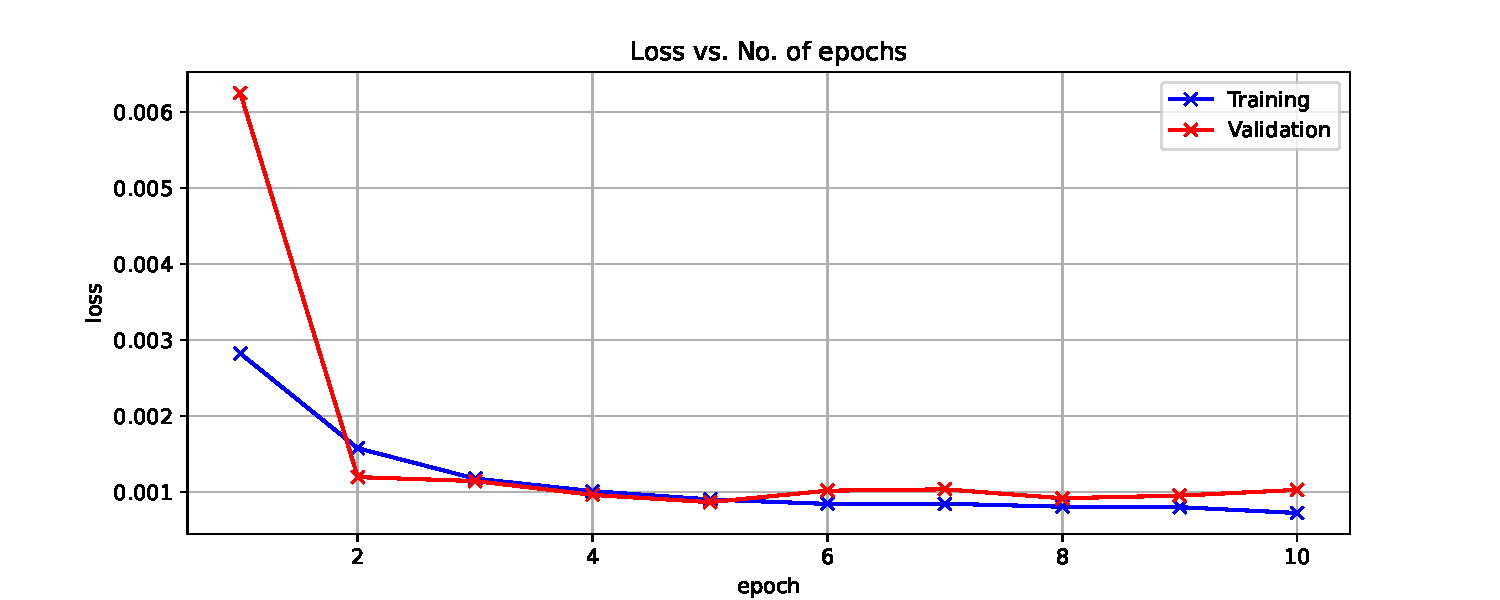
\includegraphics[width=160mm]{7.pdf}
\end{tabular}
\caption{Зависимость ошибки от номера эпохи на обучении}
\label{fig:mist}
\end{figure}

После обучения модели на 10 эпохах необходимо было подобрать пороги для каждой из размерностей с помощью алгоритма POT. У данного алгоритма есть гиперпараметр, который прямо коррелирует с тем, какой процент точек будет принят аномальными. Наша гипотеза заключается в том, что для нейтральных данных процент таких точек должен быть очень мал, исходя из чего данный параметр был подобран таким образом, чтобы на нейтральных тестовых данных доля аномальных точек не превосходила пяти процентов. 

Для тестовых данных для каждой временной точки на основе порога можно получить ответ алгоритма --- является ли данная точка аномальной или нет. Как было упомянуто ранее, разметка для сигналов ЭЭГ отсутствует, поэтому для оценки качества полученного решения были использованы косвенные метрики.

\begin{figure}[h]
\begin{tabular}{cc}
  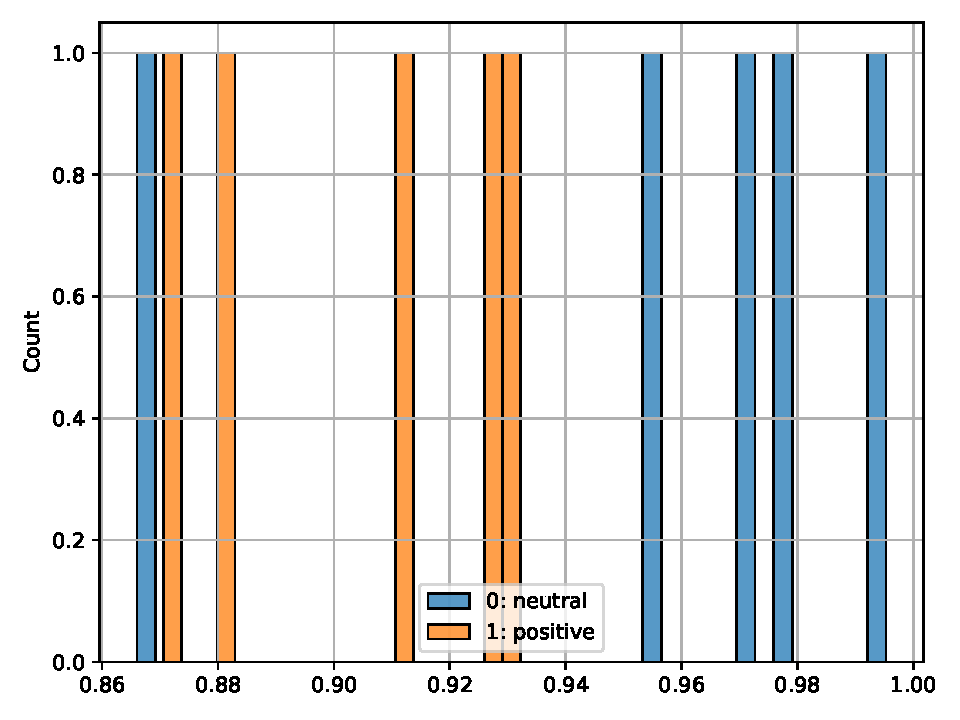
\includegraphics[width=160mm]{8.pdf}
\end{tabular}
\caption{Распределение процентов неаномальных точек для объектов тестовой выборки}
\end{figure}

Таким образом, AUC ROC модели, получающей оценки принадлежности нейтральному классу описанным выше способом будет равен 0.8, что подтверждает эффективность предложенного решения. Общий процент аномальных точек в тестовых данных для нейтрального класса будет 5, а для положительного 10, что дополнительно демонстрирует, что модель научилась различать тенденции в рядах ЭЭГ, вызванных положительной сценой, от тенденций, вызванных нейтральной сценой.

\subsection{Анализ выявленных аномалий}
\begin{figure}[h]
\begin{tabular}{cc}
  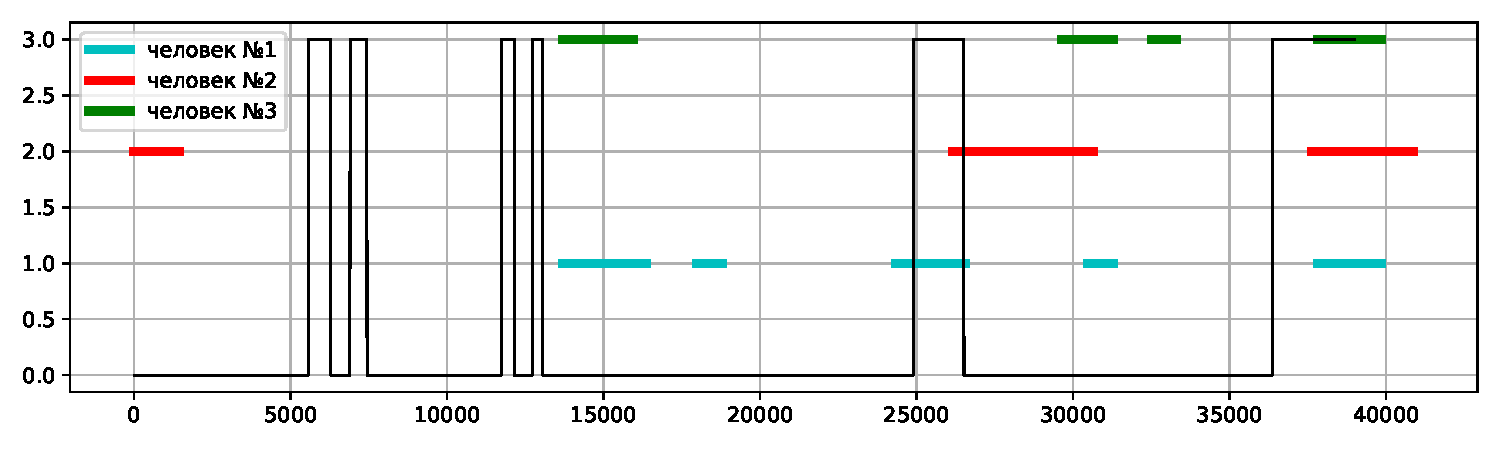
\includegraphics[width=160mm]{10.pdf}
\end{tabular}
\caption{Результаты независимых экспертов}
\label{fig:experts}
\end{figure}

Для того чтобы проинтерпретировать полученные результаты, рассмотрим реальный фрагмент положительной сцены из фильма "Затерянные в Таиланде" \; 2012 года, используемый в тестовых данных. 

\begin{figure}[h]
\begin{tabular}{cc}
  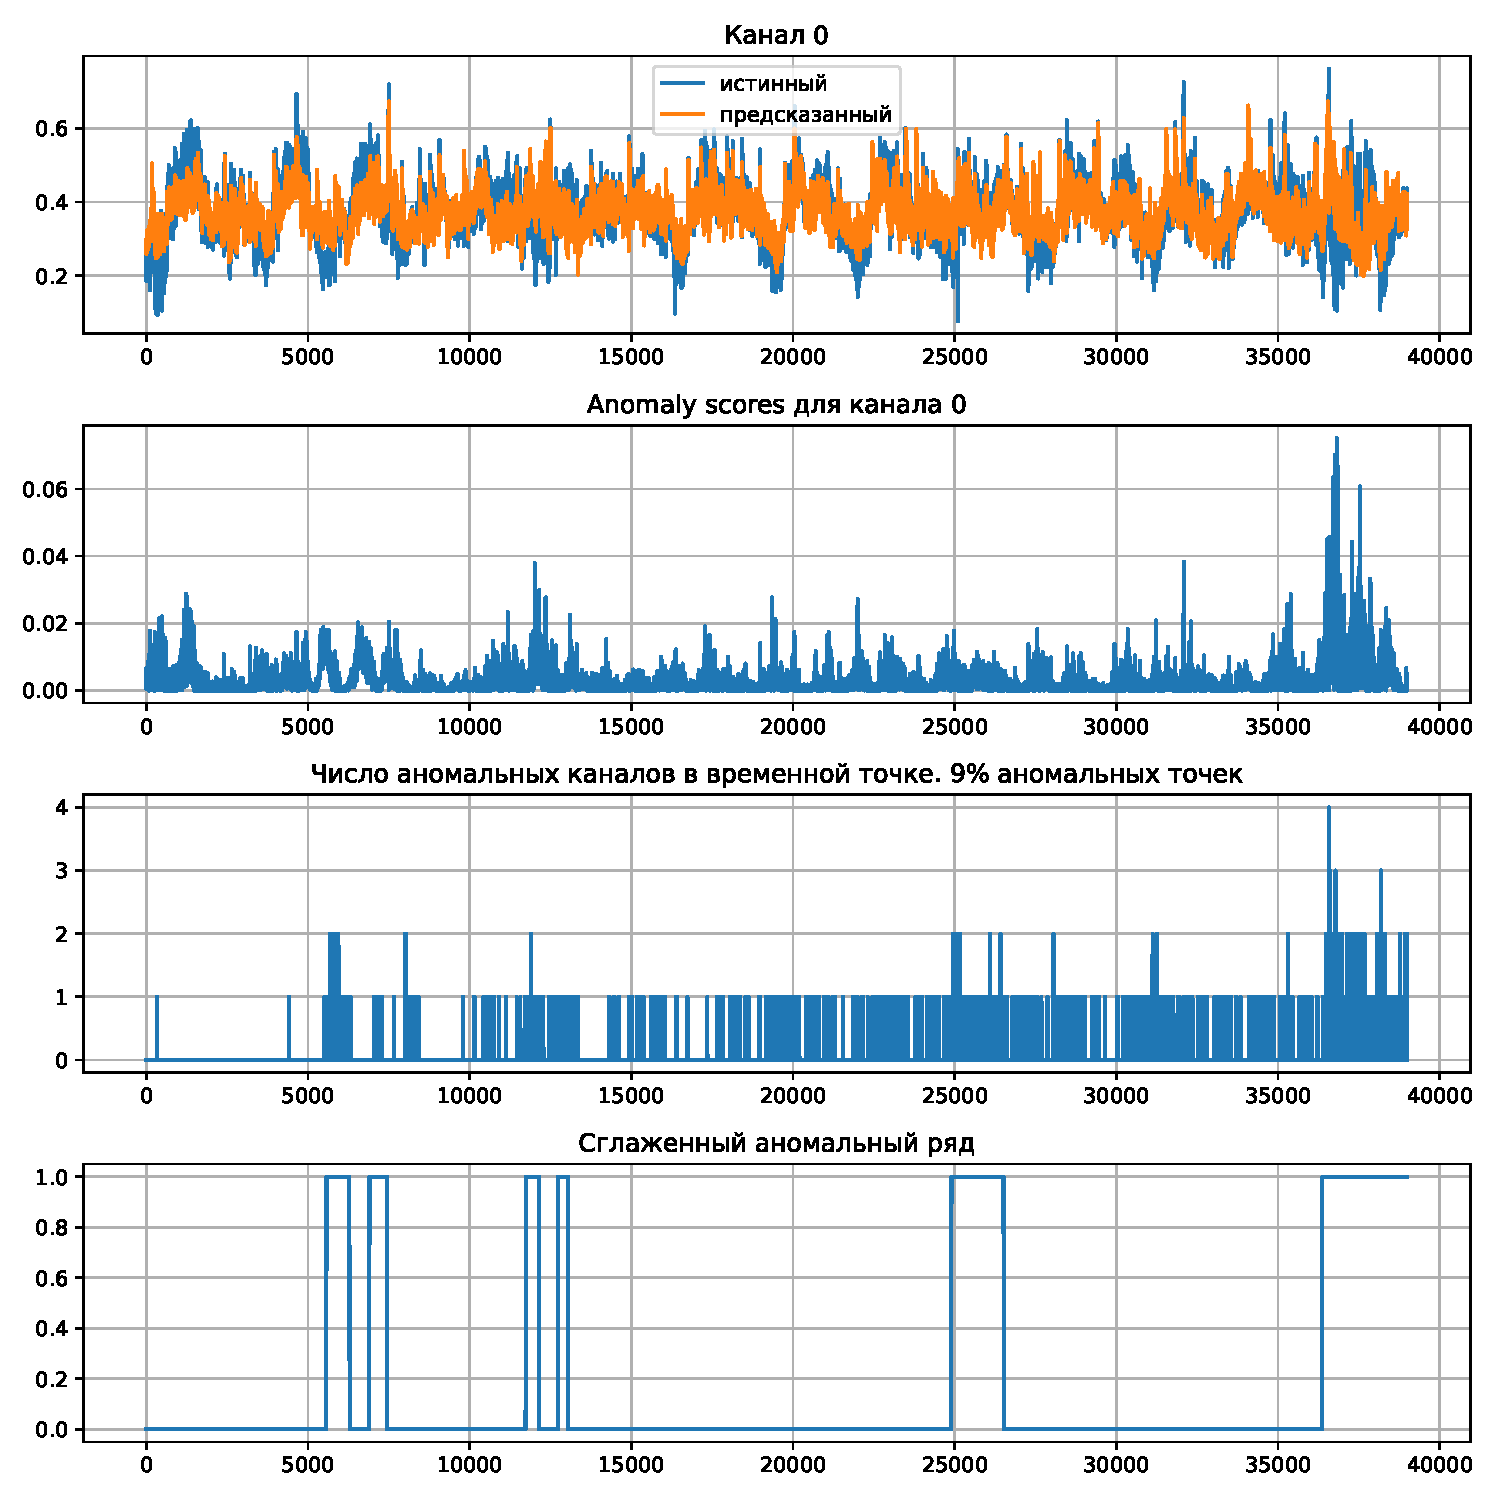
\includegraphics[width=160mm]{9.pdf}
\end{tabular}
\caption{Результаты работы алгоритма на положительном примере}
\label{fig:pos}
\end{figure}

Задача заключается в нахождении моментов, которые вызывают у зрителя самые яркие эмоции. Яркая эмоция обычно бывает непрерывной во времени, поэтому к массиву, в котором сохранены число аномальных каналов в данной временной точке, применяется сглаживание. Используется следующая эвристика: временную точку $t$ будем считать аномальной, если в окрестности в 200 временных отсчетов по крайней мере 50 точек являются аномальными. Благодаря данному преобразованию был получен график, представленный на рисунке \ref{fig:pos}. 


Для того чтобы определить адекватность полученных результатов трем независимым экспертам, не имеющим представлений о задаче, было предложено просмотреть данный фрагмент, переведенный на русский язык, и выделить отрезки, которые вызвали у них самые сильные эмоции. Полученные результаты представлены на рисунке \ref{fig:experts}.

Можно заметить, что все эксперты выделили практически один и тот же временной отрезок в конце сцены. Данный фрагмент соответствует самой смешной шутке в сцене. Модель также успешно справилась с этим отрезком и детектировала его.


\section{Выводы}
В данной работе были получены следующие результаты:
\begin{enumerate}
    \item Исследованы различные методы детектирования аномалий, проанализированы сильные и слабые стороны каждого из подходов.

    \item  Подобраны и проанализированы данные, подходящие под решение поставленной задачи.

    \item Была создана собственная реализация алгоритма, описанного в статье. Был применен новый подход к выявлению эмоций на основе детектирования аномалий, который продемонстрировал интерпретируемые результаты.
\end{enumerate}
    
\bibliographystyle{unsrtnat}
\bibliography{references}

\end{document}
